\chapter{自进化强化学习系统设计与实现}

本章描述第四章各机制的工程实现。全章先给出系统总体架构，再依次介绍沙箱环境与状态管理、跨步状态继承、推理与训练异步调度、采样与训练解耦、数据处理流程、训练监控与自动终止，最后给出系统运行流程。

\section{系统总体架构}

系统总体架构如图~\ref{fig:architecture} 所示。系统由三个协同智能体（执行者、观察者、提问者）、沙箱环境、外部冻结裁判、以及 GRPO 训练器组成，通过强化学习框架的官方注入点接入自定义采样与选组层，不 fork 框架源码。

\begin{figure}[htbp]
    \centering
    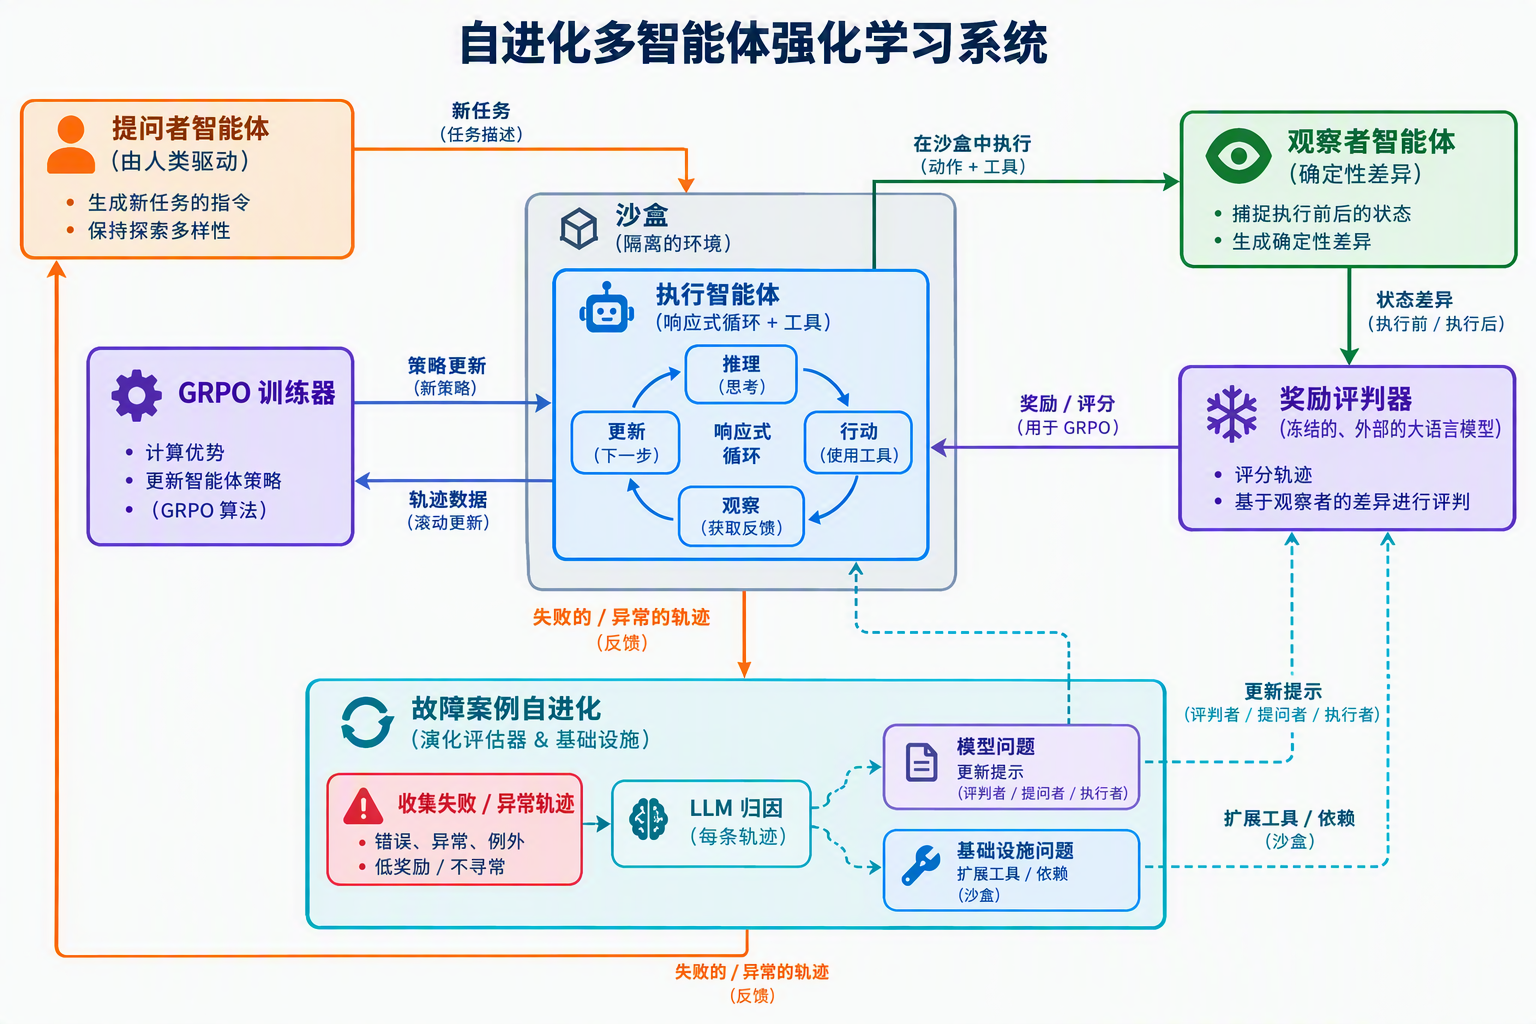
\includegraphics[width=\textwidth]{figures/fig_fig1_architecture_zh.png}
    \caption{系统总体架构}
    \label{fig:architecture}
\end{figure}

\section{沙箱环境与状态管理}

沙箱环境是自进化闭环的物理基础，其状态管理机制如图~\ref{fig:sandbox_env} 所示。系统在代码沙箱中执行 ReAct 工具调用，并在执行前后对沙箱状态各拍一次快照，作差得到确定性状态差分。状态差分包含文件系统变更（创建／修改／删除的文件及其内容）与系统状态变更（安装的包、开启的端口、启动的进程）。沙箱后端经统一契约与注册表解耦，本地开发与云端生产可零改切换。

\begin{figure}[htbp]
    \centering
    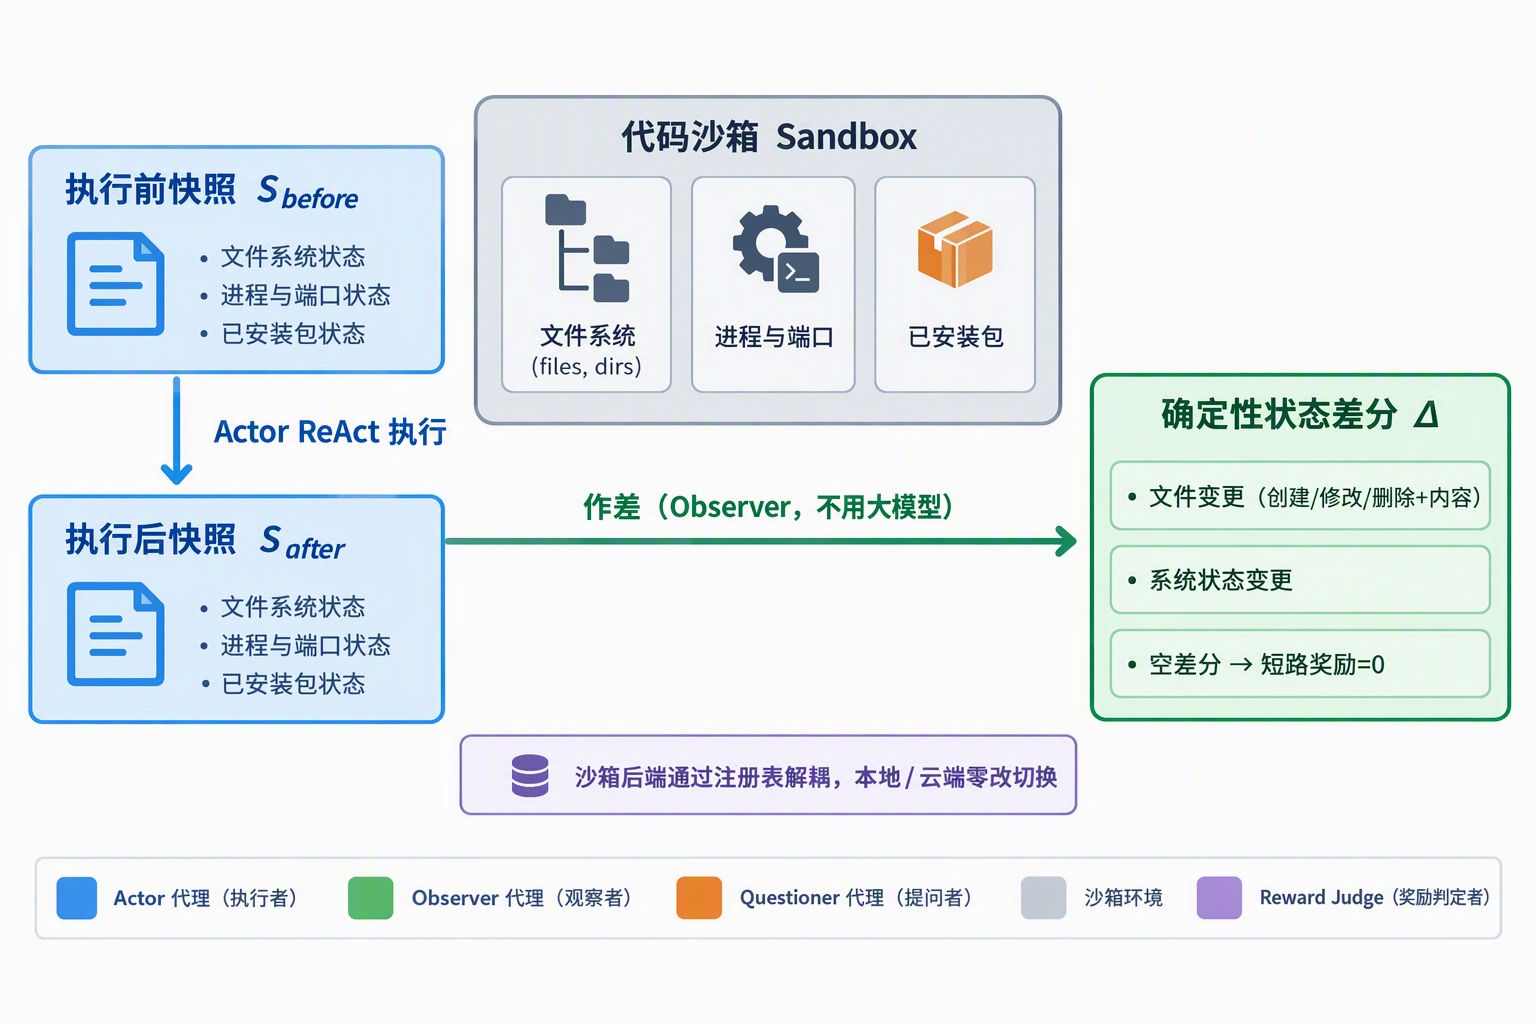
\includegraphics[width=0.85\textwidth]{figures/fig_fig18_sandbox_env_zh.png}
    \caption{沙箱环境与状态管理：执行前后快照作差得到确定性状态差分}
    \label{fig:sandbox_env}
\end{figure}

\textbf{实现与思路。} 沙箱状态的捕获由观察者（observer）负责，采用"执行前注入探针、执行后再次探针、取差集"的三步流程。文件系统探针递归遍历沙箱根目录，记录每个文件的路径、大小、修改时间及内容哈希；系统状态探针通过 \texttt{pip list}、\texttt{ss -lnp}、\texttt{ps aux} 等命令捕获已安装包、监听端口与活跃进程。两次探针的差集即为确定性状态差分，不依赖大模型，保证取证的客观性与不可操纵性。若状态差分为空（即智能体的执行对沙箱无任何可见变更），系统将该轨迹的奖励短路置 0，以此从机制上惩罚"只说不做"的奖励作弊行为。沙箱后端实现了统一的注册表接口，本地 Docker 沙箱与云端（腾讯云）沙箱通过同一接口接入，训练配置中只需切换后端标识即可实现零改切换。

\section{跨步状态继承}

跨步状态继承是自进化在环境层面的实现。系统将上轮最优轨迹的沙箱文件系统状态保存为快照，恢复到本轮新沙箱，使智能体在上轮产出的文件基础上继续工作。沙箱状态继承机制如图~\ref{fig:sandbox_inherit} 所示。

\begin{figure}[htbp]
    \centering
    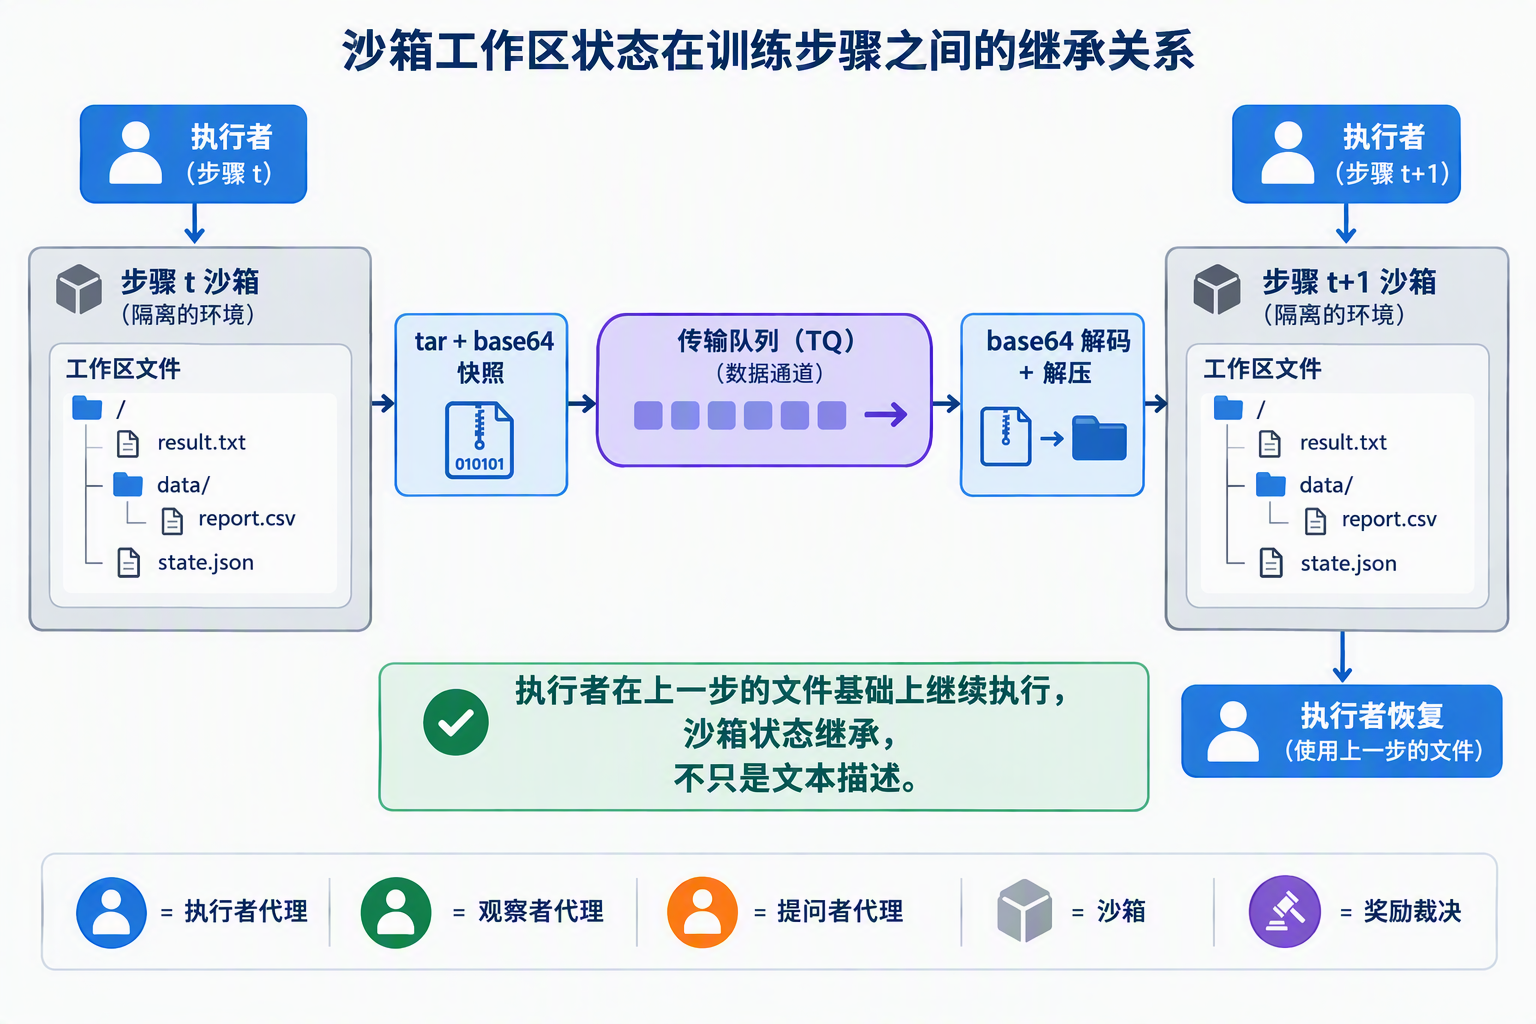
\includegraphics[width=0.85\textwidth]{figures/fig_fig6_sandbox_inherit_zh.png}
    \caption{沙箱状态继承机制}
    \label{fig:sandbox_inherit}
\end{figure}

\section{推理与训练异步调度}

推理与训练异步分离编排，调度时序如图~\ref{fig:async_schedule} 所示：rollout 阶段推理引擎独占 GPU，训练阶段推理让出；权重更新后异步同步回推理引擎。这一设计使推理与训练互不阻塞，提升系统吞吐。

\begin{figure}[htbp]
    \centering
    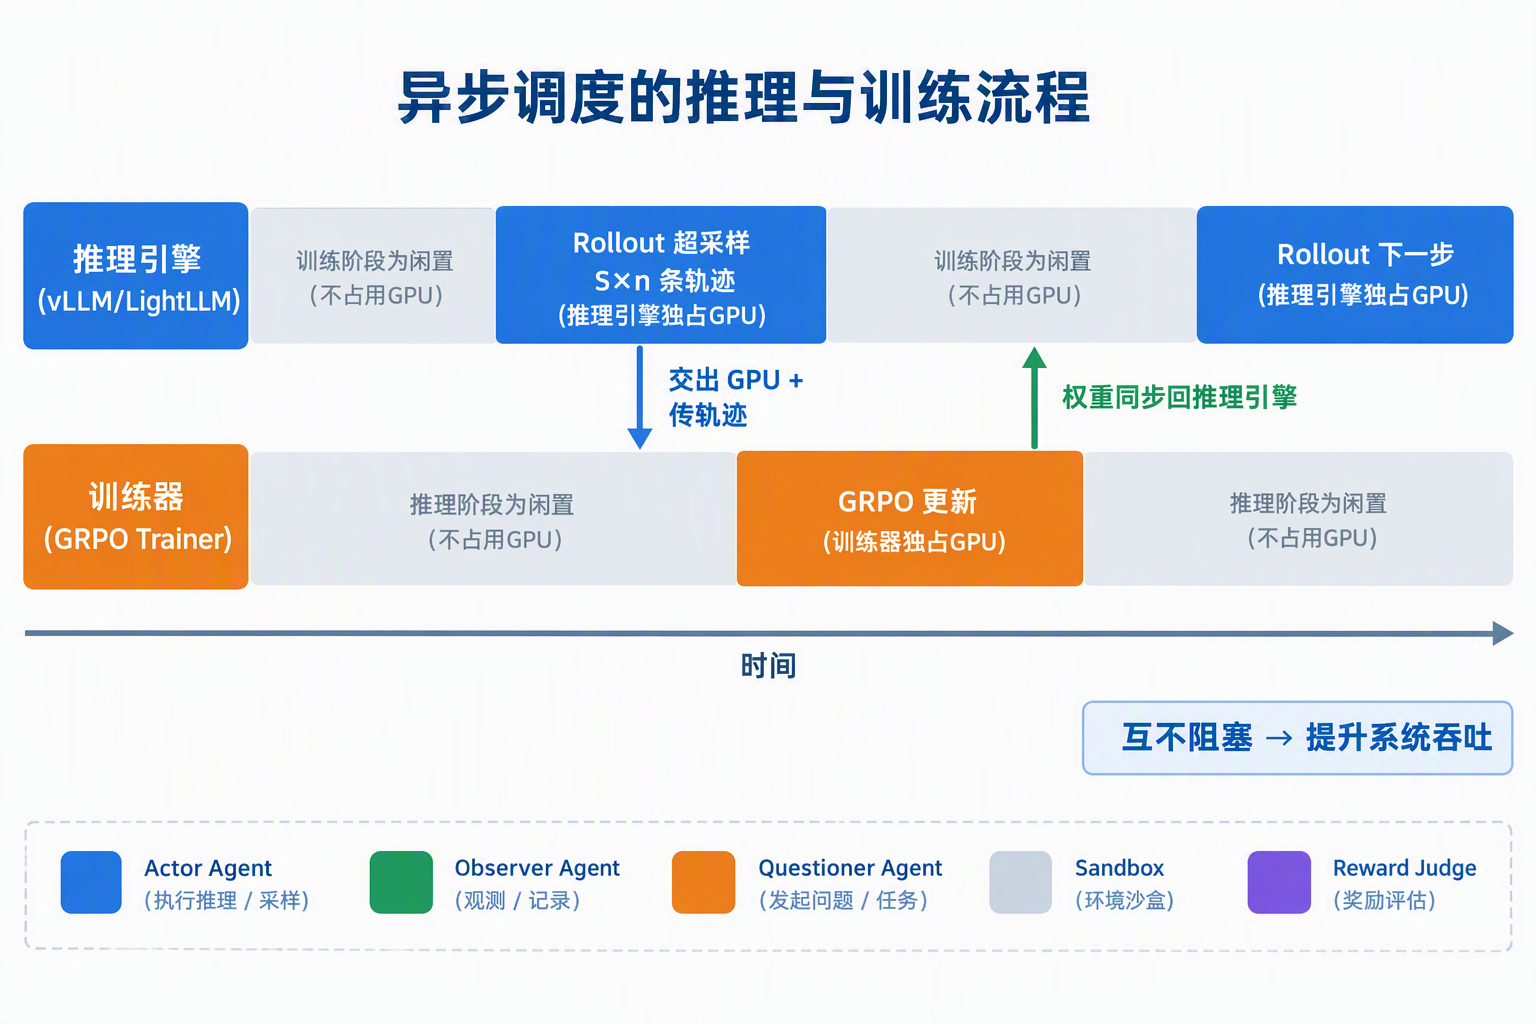
\includegraphics[width=0.9\textwidth]{figures/fig_fig19_async_schedule_zh.png}
    \caption{推理与训练异步调度时序：两阶段交替独占 GPU，权重更新后同步回推理引擎}
    \label{fig:async_schedule}
\end{figure}

\textbf{实现与思路。} 系统基于 verl（HybridFlow）框架的 HYBRID 模式接入，该模式下推理引擎（LightLLM）在 rollout 阶段持有完整的 KV 缓存与权重显存，训练阶段主动释放（\texttt{release\_memory\_occupation}），将 GPU 显存归还给训练器。权重更新完成后，训练器将最新的模型参数广播回推理引擎，推理引擎重新加载并准备下一步 rollout。这一流程完全通过框架官方钩子实现，无需 fork 源码。GPU 显存峰值出现在 rollout 阶段（推理引擎保持 KV 缓存），因此推理引擎的显存占用比例（\texttt{gpu\_memory\_utilization}）是影响训练可行性的关键参数，需在推理吞吐与训练可用显存之间取得平衡。

\section{采样与训练解耦}

多智能体协作采样、超采样-淘汰-选组、跨步种子生成等环节需在强化学习框架的定长批次约束下无缝衔接。系统通过框架的官方注入点接入自定义采样管理器与选组层，将 $S \times n$ 条超采样轨迹收敛到 $N \times n$ 条训练批次，如图~\ref{fig:decouple} 所示。

\begin{figure}[htbp]
    \centering
    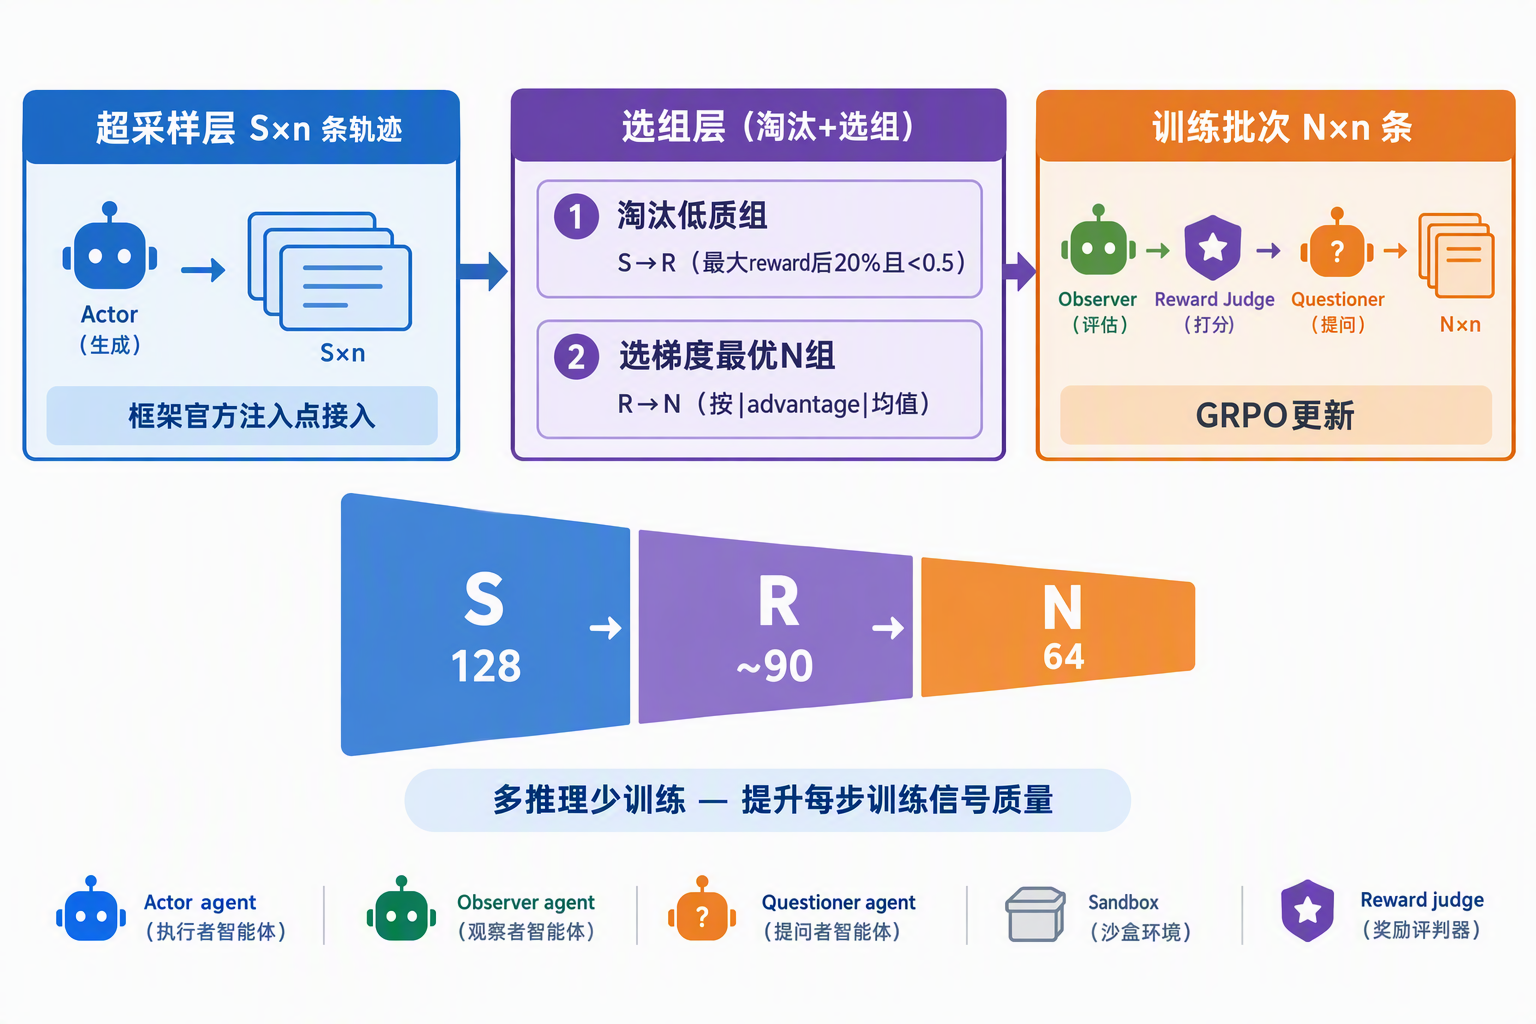
\includegraphics[width=0.85\textwidth]{figures/fig_fig20_decouple_zh.png}
    \caption{采样与训练解耦：超采样层 → 选组层 → 训练批次，漏斗式收敛}
    \label{fig:decouple}
\end{figure}

\textbf{实现与思路。} 采样管理器负责组织超采样的 $S \times n$ 条轨迹——其中 $S$ 为当前步的超采样量（初始为 $2N$，随淘汰动态收缩），$n$ 为 GRPO 组大小。选组层作为框架的后处理钩子，在优势计算之后、策略梯度更新之前介入：首先对所有组按淘汰判据（最大 reward 在后 20\% 且 $< 0.5$）过滤，得到 $R$ 个存活组；再按组内优势绝对值均值降序排列，取前 $N$ 组进入最终训练批次。这一漏斗式流程的关键在于框架不感知"多采少训"的存在——训练器始终看到固定的 $N \times n$ 批次，自进化的额外采样与过滤对框架完全透明。

\section{自进化数据处理流程}

一个训练步内的完整数据处理流程如图~\ref{fig:data_pipeline} 所示：采样管理器组织种子任务并驱动执行者 rollout；观察者在每条轨迹执行前后拍快照并计算状态差分；裁判据差分打分并写回奖励；选组层淘汰低质组、选梯度最优组；训练器用选中批次做 GRPO 更新；训练步结束后，跨步模块对存活组产生下一轮种子。

\begin{figure}[htbp]
    \centering
    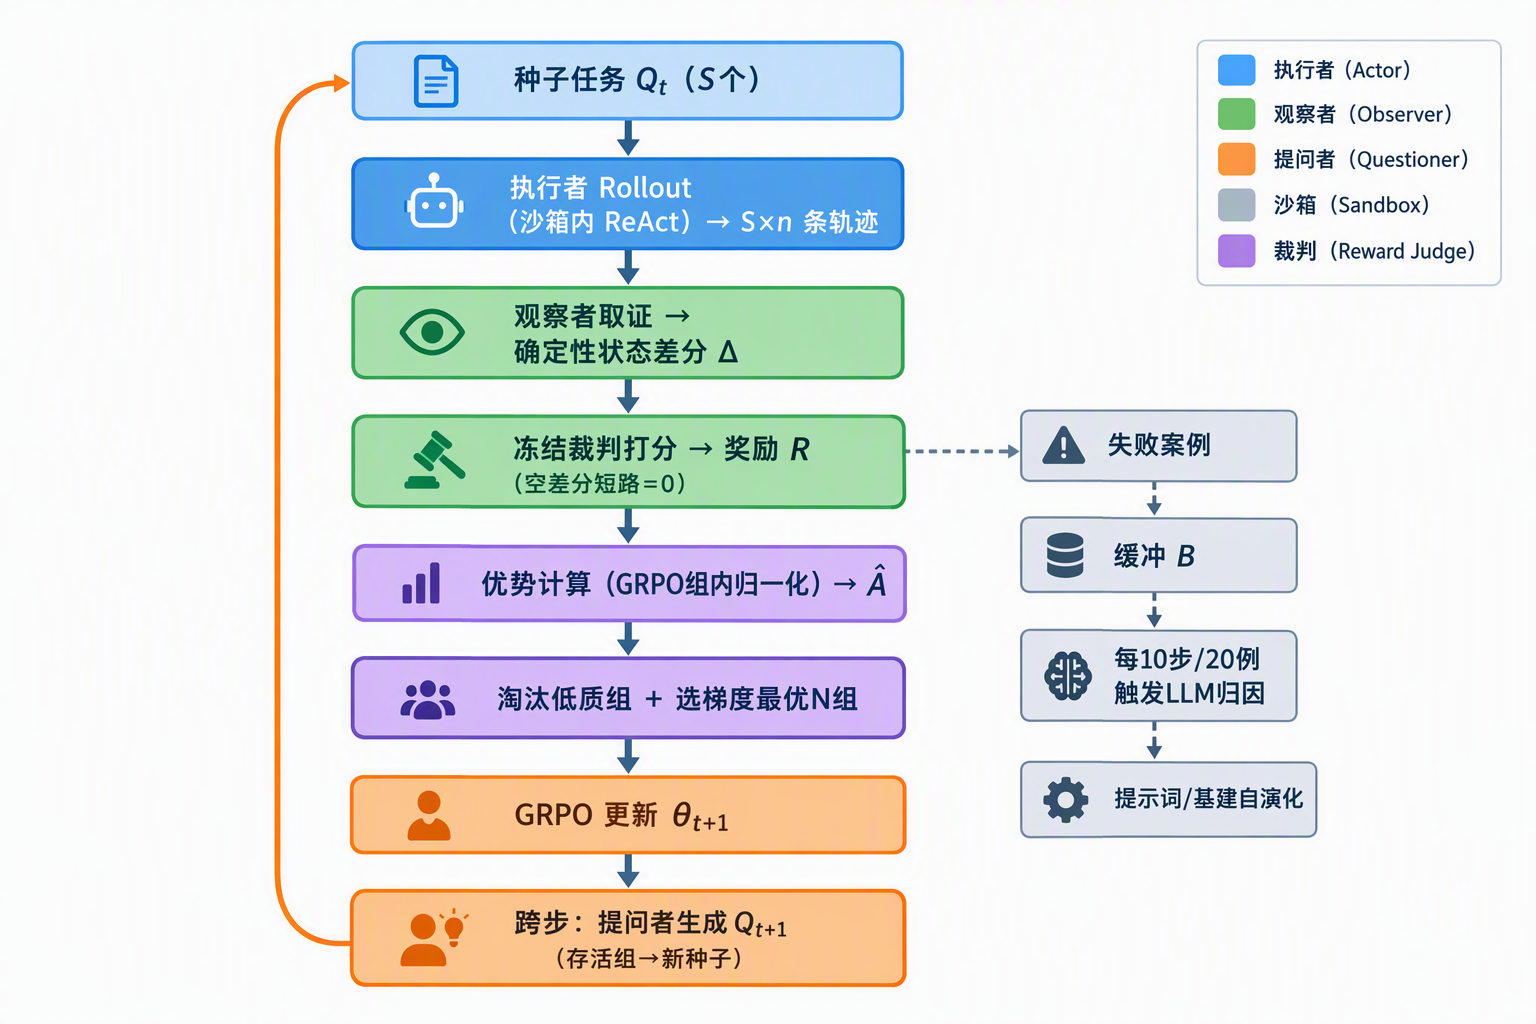
\includegraphics[width=0.75\textwidth]{figures/fig_fig21_data_pipeline_zh.png}
    \caption{单训练步内的自进化数据处理流程}
    \label{fig:data_pipeline}
\end{figure}

\textbf{实现与思路。} 数据处理流程的核心设计原则是"各环节单向流动、无回路依赖"：种子 → rollout → 取证 → 打分 → 选组 → 更新 → 下一轮种子，每个环节只依赖上一步的输出，便于各环节独立测试与替换。失败案例缓冲（\texttt{BadcaseBuffer}）作为旁路挂接在打分环节之后：每条奖励低于阈值、含 agent\_error 或空交付的轨迹会被异步收集；每 10 步或累积 20 条失败案例时，触发 LLM 归因流程（\texttt{LLMAttribution}），根据归因结果分别更新提示词或扩展基建，再清空缓冲、开始下一周期的收集。这一旁路设计保证失败案例自演化不阻塞主训练流程，任何归因或更新的失败都以 best-effort 方式处理、不影响训练继续推进。

\section{训练监控与自动终止}

第四章界定了自进化稳定性的判据指标，本节描述其工程实现。系统在每个训练步的优势计算完成后，实时采集以下坍缩指标并写入训练日志：

\begin{itemize}
    \item 奖励标准差（sys/reward\_std）：组内奖励的标准差。
    \item 优势标准差（sys/advantage\_std）：优势的标准差。
    \item 组内奖励标准差（sys/group\_reward\_std）：GRPO 组内奖励的标准差，0 表示退化组。
    \item 策略 KL 散度（actor/ppo\_kl）：策略偏离参考策略的程度。
    \item 训练损失（actor/pg\_loss）：出现 NaN／Inf 表示训练崩溃。
    \item 存活组数（sys/num\_groups）：淘汰后的存活组数。
\end{itemize}

自动终止判据如下：奖励标准差 $< 10^{-6}$（策略多样性坍缩）；优势标准差 $< 10^{-6}$（无梯度信号）；训练损失为 NaN 或 Inf（训练崩溃）；策略 KL 散度 $> 10$（策略偏离过远）；存活组数 $<$ 训练组数 $N$（超采样池耗尽）。任一判据触发时，系统跳过跨步种子生成，训练循环在下一步检测到终止标志后退出。训练指标与终止判据如图~\ref{fig:training_curves} 所示。

\begin{figure}[htbp]
    \centering
    
\includegraphics[width=0.9\textwidth]{figures/fig_fig9_training_curves_zh.png}
    \caption{训练指标与终止判据（奖励均值、奖励标准差、pg\_loss、ppo\_kl）}
    \label{fig:training_curves}
\end{figure}

\section{系统运行流程}

综合以上模块，系统的完整运行流程为：初始化沙箱后端、推理引擎、训练器与奖励回路；第一步从初始种子采样，后续步用跨步生成的种子；每步内经过 rollout、状态差分取证、奖励打分、淘汰选组、GRPO 更新、训练监控、跨步种子生成；每 10 步或攒够 20 个失败案例时触发一次评估器与基建的自演化；直至终止判据触发或达到步数上限。完整流程如算法~\ref{alg:main_loop} 所示。

\begin{algorithm}[htbp]
\caption{自进化强化学习主循环（含失败案例自演化）}
\label{alg:main_loop}
\begin{algorithmic}[1]
\Require 初始种子集 $Q_0$，训练组数 $N$，组大小 $n$，最大步数 $T_{\max}$
\Ensure 训练后的策略 $\pi_\theta$
\State 初始化沙箱后端、推理引擎、训练器、奖励回路；$\pi_\theta \gets \pi_{\theta_0}$
\State $S \gets 2N$；\ 种子集 $Q \gets Q_0$；\ 失败案例缓冲 $\mathcal{B} \gets \emptyset$ \Comment{第一步冷启动}
\For{$t = 0$ \textbf{to} $T_{\max}-1$}
    \State $\{\tau_{ij}\} \gets \textproc{Rollout}(\pi_\theta, Q, n)$ \Comment{$S$ 组 $\times\,n$ 条，沙箱内 ReAct}
    \For{\textbf{each} 轨迹 $\tau_{ij}$}
        \State $d_{ij} \gets \textproc{Observe}(\tau_{ij})$ \Comment{执行前后状态差分（确定性取证）}
        \State $r_{ij} \gets \textproc{Judge}(d_{ij})$ \Comment{冻结裁判据差分打分；空差分短路为 0}
        \If{$\textproc{IsFailed}(\tau_{ij}, d_{ij}, r_{ij})$} \Comment{失败/异常/自述与差分矛盾}
            \State $\mathcal{B} \gets \mathcal{B} \cup \{(\tau_{ij}, d_{ij}, r_{ij})\}$ \Comment{收集失败案例}
        \EndIf
    \EndFor
    \State $\{\hat{A}_{ij}\} \gets \textproc{ComputeAdvantage}(\{r_{ij}\})$ \Comment{GRPO 组内归一化}
    \State $m \gets \textproc{CollapseMetrics}(\{r_{ij}\}, \{\hat{A}_{ij}\})$ \Comment{奖励/优势标准差等}
    \If{$\textproc{ShouldStop}(m)$} \Comment{坍缩或崩溃判据触发}
        \State \textbf{break}
    \EndIf
    \State $\mathcal{R} \gets \textproc{Eliminate}(\{r_{ij}\})$ \Comment{$S \to R$：丢最大 reward 后 20\% 且 $<0.5$ 的组}
    \State $\mathcal{S} \gets \textproc{Select}(\mathcal{R}, N)$ \Comment{$R \to N$：按 $|\hat{A}|$ 均值选梯度最强 $N$ 组}
    \State $\pi_\theta \gets \textproc{GRPOUpdate}(\pi_\theta, \mathcal{S})$ \Comment{仅 $N\times n$ 条进梯度}
    \If{$(t+1) \bmod 10 = 0$ \textbf{or} $|\mathcal{B}| \ge 20$} \Comment{触发失败案例自演化}
        \State $(\Delta_{\text{prompt}}, \Delta_{\text{infra}}) \gets \textproc{LLMAttribution}(\mathcal{B})$ \Comment{大模型归因：模型/基建}
        \State $\textproc{UpdatePrompts}(\Delta_{\text{prompt}})$ \Comment{热更新裁判/提问者/执行者提示词}
        \State $\textproc{ExpandInfra}(\Delta_{\text{infra}})$ \Comment{动态注册工具/补依赖/修 harness}
        \State $\mathcal{B} \gets \emptyset$ \Comment{清空缓冲，开始下一周期收集}
    \EndIf
    \State $Q \gets \textproc{Questioner}(\textproc{Summary}(\mathcal{R}),\ \textproc{Snapshot}(\mathcal{R}))$ \Comment{跨步：存活组产下一轮种子}
    \State $S \gets |\mathcal{R}|$ \Comment{下一步超采样量 $S=R$，随淘汰动态收缩}
\EndFor
\State \Return $\pi_\theta$
\end{algorithmic}
\end{algorithm}

三智能体的协作时序如图~\ref{fig:sequence} 所示，执行者的沙箱内 ReAct 循环如图~\ref{fig:react_loop} 所示。

\begin{figure}[htbp]
    \centering
    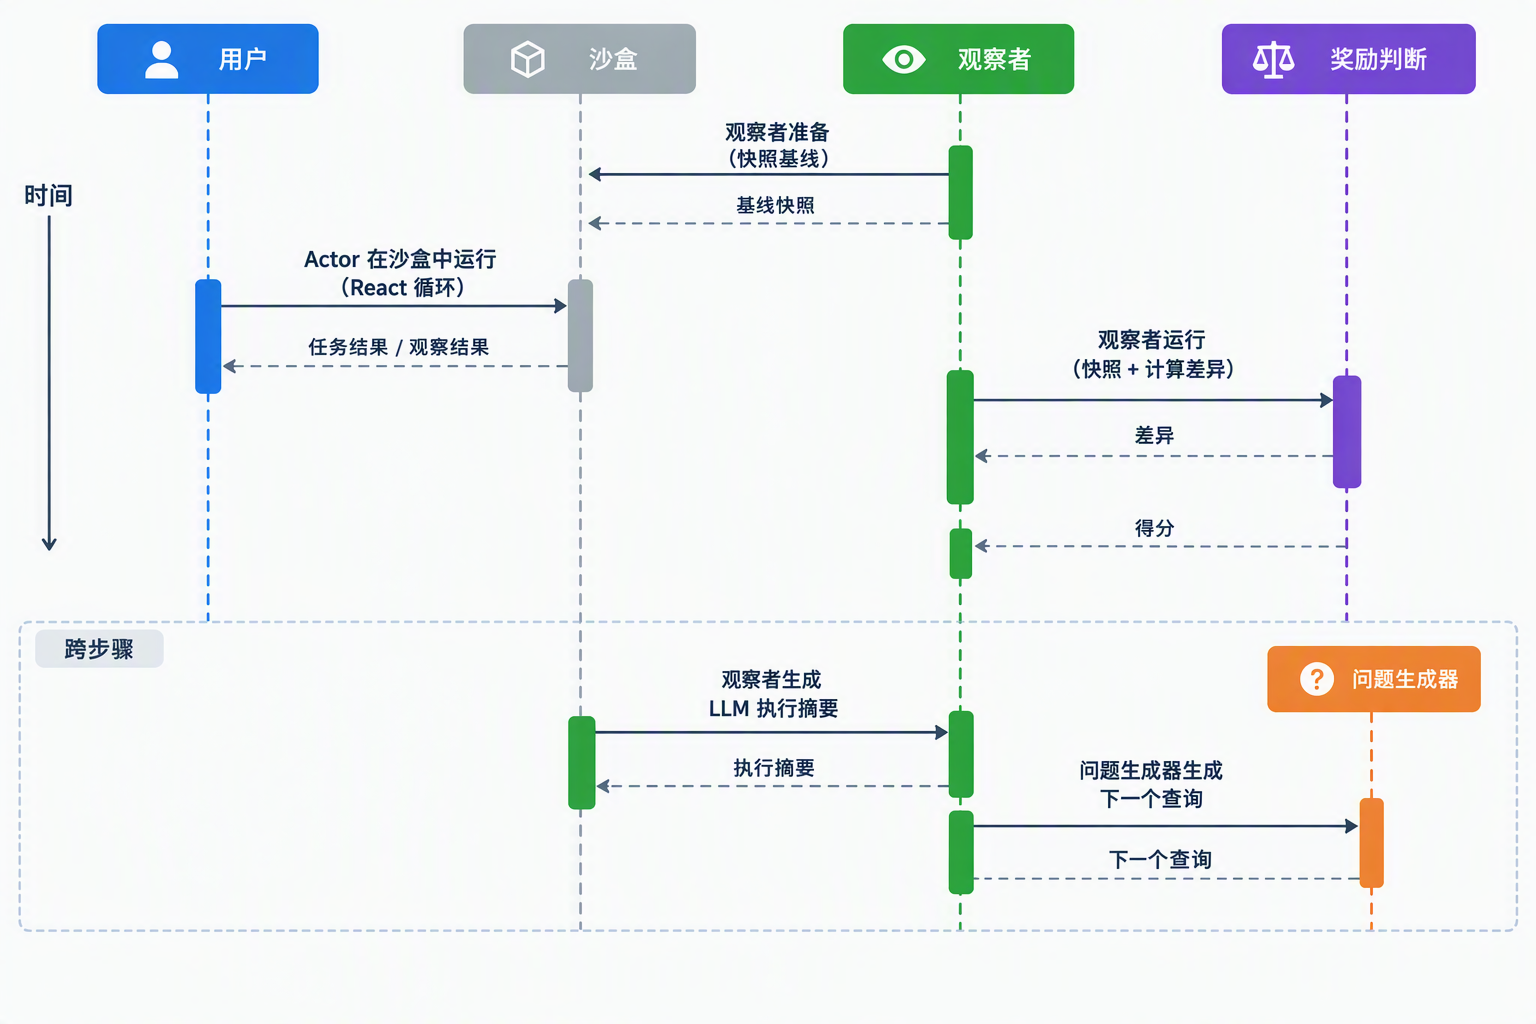
\includegraphics[width=0.85\textwidth]{figures/fig_fig7_sequence_zh.png}
    \caption{三智能体协作时序}
    \label{fig:sequence}
\end{figure}

\begin{figure}[htbp]
    \centering
    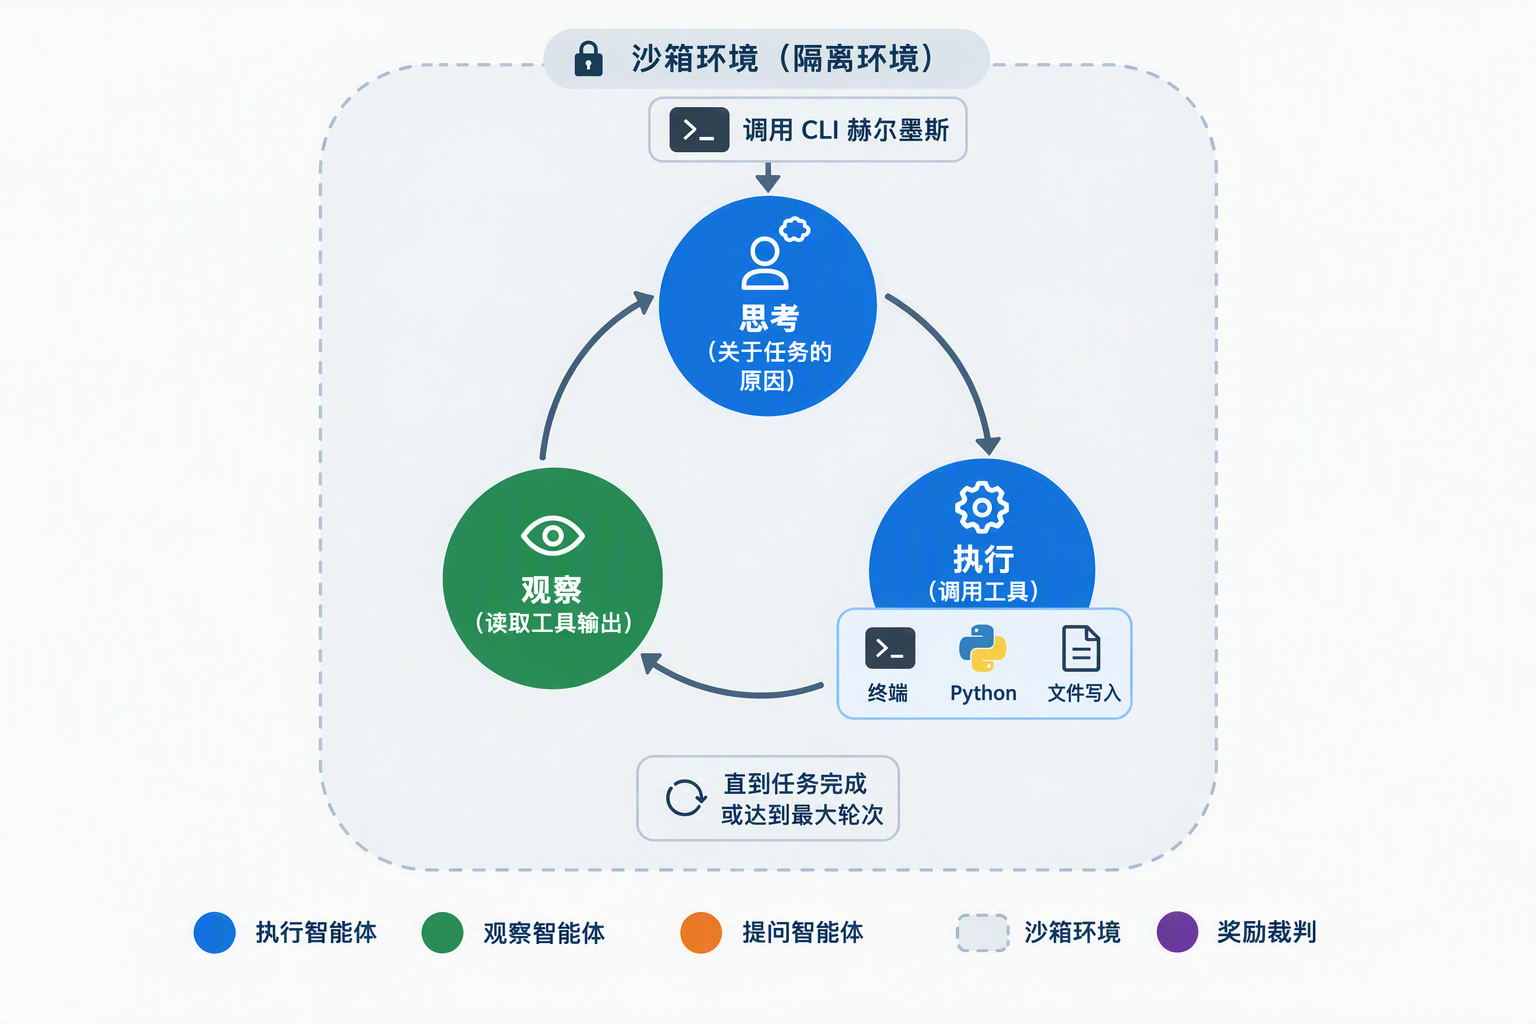
\includegraphics[width=0.7\textwidth]{figures/fig_fig8_react_loop_zh.png}
    \caption{执行者沙箱内 ReAct 循环}
    \label{fig:react_loop}
\end{figure}

\section{本章小结}

本章描述了系统的工程实现：系统总体架构、沙箱环境与状态管理、跨步状态继承、推理与训练异步调度、采样与训练解耦、数据处理流程、训练监控与自动终止，以及完整的系统运行流程。这些工程模块共同保证第四章各机制得以物理运转，并使自进化过程稳定可控。
